% DO NOT COMPILE THIS FILE DIRECTLY!
% This is included by the other .tex files.
\section*{Background}
\begin{frame}[t,plain]
\titlepage
\end{frame}
%%%%%%%%%%%%%%%%%%%%%%%%%%%%%%%%%%%
%%%%%%%%%%%%%%%%%%%%%%%%%%%%%%%%%%%
\begin{frame}{Logarithmic pooling -- Motivation}
 \begin{itemize}
  \item Obtain important insights on consensus belief formation and group decision making~\citep{genest1986B};
  \begin{figure}
 \begin{center}
  
\includegraphics[scale=0.3]{figures/Consensus.jpg}
 \end{center}
  \end{figure}
  \item Applications in a range of fields, from infectious disease modelling~\citep{Coelho2009} and wildlife conservation~\citep{poole2000} to engineering~\citep{savchuk1994};
  \item[\tikzmark{bl}\textbullet] BUT how to give each expert/information source a weight without being (totally) arbitrary? \tikzmark{br}
 \end{itemize}
 \tikz[overlay,remember picture]{\draw[red]
  ($(bl)+(-1.2em,0.9em)$) rectangle
  ($(br)+(22.5em,-1.3em)$);}
\end{frame}
%%%%%%%%%%%%%%%%%%%%%%%%%%%%%%%%%%%
%%%%%%%%%%%%%%%%%%%%%%%%%%%%%%%%%%%
\begin{frame}{Logarithmic pooling -- Definition \& Notation}
Let $\mathbf{F_\theta} = \{f_0(\theta), f_1(\theta), \ldots, f_K(\theta)\}$ be the set of \sout{prior} distributions representing the opinions of $K+1$ experts and let $\boldsymbol\alpha =\{\alpha_0, \alpha_1, \ldots, \alpha_K \}$ be the vector of weights, such that $\alpha_i > 0\: \forall i$ and $\sum_{i=0}^K \alpha_i = 1$.
Then the log-pooled prior is
\begin{equation}
\label{eq:logpool}
 \pi(\theta) = t(\boldsymbol\alpha) \prod_{i=0}^K f_i(\theta)^{\alpha_i} 
\end{equation}
with $t(\boldsymbol\alpha) = \int_{\boldsymbol\Theta}\prod_{i=0}^K f_i(\theta)^{\alpha_i}d\theta$.
\begin{itemize}
 \item Enjoys rather desirable properties, such as~\textit{external Bayesianity}~\citep{genest1986B};
 \item \cite{poole2000} prove that $t(\boldsymbol\alpha)$ is always finite for the case $K=1$ (2 experts/priors), which we extend for any finite $K$.
 See Theorem 1 in~\url{http://arxiv.org/pdf/1502.04206v1.pdf} for a simple proof.
\end{itemize}
\end{frame}
%%%%%%%%%%%%%%%%%%%%%%%%%%%%%%%%%%%
%%%%%%%%%%%%%%%%%%%%%%%%%%%%%%%%%%%
\begin{frame}{Maximise the entropy of $ \pi(\theta)$ }
 \begin{itemize}
  \item If there is no information about the reliabilities of the experts one might want to assign $\boldsymbol\alpha$ so as to maximise entropy of the resulting distribution:
  \begin{align*}
   H_{\pi}(\theta) &=-\int_{\boldsymbol\Theta}\pi(\theta)\ln\pi(\theta)d\theta \\
   H_{\pi}(\theta; \boldsymbol\alpha) &= \sum_{i=0}^{K} \alpha_i E_{\pi}[ - \ln f_i(\theta)] - \ln t(\boldsymbol\alpha)
  \end{align*}
  \item Formally, we want to find $\hat{\boldsymbol\alpha}$ such that
  \[\hat{\boldsymbol\alpha}:= \argmax H_{\pi}(\theta; \boldsymbol\alpha)  \]
  \item Caveats: (i) is not guaranteed to yield an unique solution; (ii) is rather prone to yield ``trivial'' solutions.
 \end{itemize}
\end{frame}
%%%%%%%%%%%%%%%%%%%%%%%%%%%%%%%%%%%
%%%%%%%%%%%%%%%%%%%%%%%%%%%%%%%%%%%
\begin{frame}{Minimise KL divergence between the $f_i$'s and $\pi(\theta)$}
\begin{itemize}
 \item What if we want to minimise conflict between the consensus and each individual opinion?
 \item Let $d_i = \text{KL}(f_i || \pi)$ and let $L(\boldsymbol\alpha)$ be a loss function such that
\begin{align*}
L(\boldsymbol\alpha) &= \sum_{i=0}^Kd_i \\
     &= -K\ln t(\boldsymbol\alpha) + \sum_{i=0}^K\sum_{j\neq i}^K\alpha_j\text{KL}(f_i||f_j) \\
     \hat{\boldsymbol\alpha}:=& \argmin L(\boldsymbol\alpha)   
\end{align*}
\item Contrary to the above, the loss function is convex, thus there is a unique solution~\citep{rufo2012A}.
\end{itemize}
\end{frame}
%%%%%%%%%%%%%%%%%%%%%%%%%%%%%%%%%%%
%%%%%%%%%%%%%%%%%%%%%%%%%%%%%%%%%%%
\begin{frame}{Place a prior on the weights}
 \begin{itemize}
  \item An appealing alternative is to place a (hyper) prior on the weights ($\boldsymbol\alpha$);
  \item Two options:\\
 (a) Dirichlet prior:
\[ \pi(\boldsymbol\alpha) = \frac{1}{\mathcal{B}(\boldsymbol X)}\prod_{i=0}^K \alpha_i^{x_i-1}\]
 (b) logistic-normal:
 \[\alpha_i = \frac{e^{m_i}}{\sum_{i=0}^{K} e^{m_i}}, \: m_i \sim N(\mu_i, \sigma_i^2)\]
 \item Advantage: accomodates uncertainty in natural way, and is very flexible;
 \item Caveat(s): may yield inconsistent results and hardly ever allows for analytical solutions.
 \end{itemize}
\end{frame}
%%%%%%%%%%%%%%%%%%%%%%%%%%%%%%%%%%%
%%%%%%%%%%%%%%%%%%%%%%%%%%%%%%%%%%%
\begin{frame}{Application: binomial probabilities}
 \begin{itemize}
  \item $Y\sim Bernoulli(\theta)$ and
  \[f_i(\theta;a_i, b_i) = \frac{\Gamma(a_i + b_i)}{\Gamma(a_i b_i)} \theta^{a_i-1}(1-\theta)^{b_i-1}\]
  \item Allows for simple expressions for the entropy and KL divergence [$\pi(\theta; \boldsymbol\alpha)$ is also Beta], and efficient sampling from the hyperpriors;
  \item \cite{savchuk1994} consider an example in which four experts are required supply prior information about the survival probability of
a certain unit for which there have been $y = 9$ successes out of $n = 10$ trials;
  \item We propose to evaluate performance using integrated (marginal) likelihoods, a.k.a., prior evidence.
 \end{itemize}
\end{frame}
%%%%%%%%%%%%%%%%%%%%%%%%%%%%%%%%%%%
%%%%%%%%%%%%%%%%%%%%%%%%%%%%%%%%%%%
\begin{frame}{\sout{very} Preliminary results}
\begin{figure}
 \begin{center}
  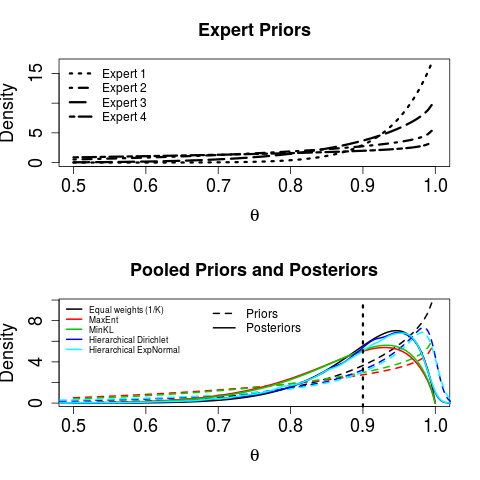
\includegraphics[scale=0.4]{figures/new_beta_example.png}
 \end{center}
\end{figure}
\end{frame}
%%%%%%%%%%%%%%%%%%%%%%%%%%%%%%%%%%%
%%%%%%%%%%%%%%%%%%%%%%%%%%%%%%%%%%%
\begin{frame}{\sout{very} Preliminary results II}
\begin{table}[ht]
\caption{Weights obtained using the three methods for the proportion estimation problem. $^1$ -- Kullback-Leibler $^2$ -- Posterior mean for $\boldsymbol\alpha$.}
\centering
\begin{tabular}{ccccc}
  \hline
Method  & $\alpha_0$ & $\alpha_1$ & $\alpha_2$ & $\alpha_3$ \\ 
  \hline
Maximum entropy & 0.00 & 1.00 & 0.00 & 0.00 \\ 
Minimum KL$^1$ divergence& 0.04 & 0.96 & 0.00 & 0.00 \\ 
Hierarchical prior$^2$ & 0.26 & 0.24 & 0.26 & 0.23 \\ 
   \hline
\end{tabular}
\end{table}
\begin{table}[ht]
\caption{Integrated likelihoods for the priors of each expert as well as the combined priors.
$^1$ Calculated using the posterior mean of $\boldsymbol\alpha$}
\centering
\begin{tabular}{cccc}
   \hline
   \multicolumn{2}{c}{Expert priors} &  \multicolumn{2}{c}{Pooled priors} \\
   \hline
   Expert 0 & 0.237 & Equal weights & 0.254\\
   Expert 1 & 0.211 & Maximum entropy & 0.211 \\
   Expert 2 & 0.256 & Minimum KL & 0.223\\ 
   Expert 3 & 0.163 & Hierarchical$^1$ & 0.255 \\
   \hline
\end{tabular}
\end{table}
\end{frame}
%%%%%%%%%%%%%%%%%%%%%%%%%%%%%%%%%%%
%%%%%%%%%%%%%%%%%%%%%%%%%%%%%%%%%%%
\begin{frame}{Partial Sum up}
\begin{itemize}
 \item Our results are not yet decisive regarding which method is better;
 \item The Dirichlet approach seems the most natural from a Bayesian perspective, but prior sensitivity is currently unknown;
%  \item Generalise the hyperprior approach to the exponential family;
%  \item The relationship between the integrated likelihood of the combined (pooled) distribution in relation to that of each individual distribution.
%  \item Applications to dynamic models~\citep{poole2000}.
%  $l_i(y) = \int_{\boldsymbol\Theta}f(\theta|y)\pi_i(\theta)d\theta$ and $l(y; \boldsymbol\alpha) = \int_{\boldsymbol\Theta}f(\theta|y)\pi(\theta; \boldsymbol\alpha)d\theta$.
\end{itemize}
\end{frame}
%%%%%%%%%%%%%%%%%%%%%%%%%%%%%%%%%%%
%%%%%%%%%%%%%%%%%%%%%%%%%%%%%%%%%%%
\begin{frame}{Induce-then-pool or pool-then-induce?}
\begin{itemize}
 \item Let $\theta \in \Theta \subseteq \mathbb{R}^p$ and $y \in \mathcal{Y} \subseteq \mathbb{R}^p$ and define the model (transformation) as $M \,:\, \Theta \to \mathcal{Y}$.
 \item Finally recall $\mathbf{F_\theta}$ is a set of $K$ distributions on $\theta$.
 \item We may want to gain insight into $y$, even though we only have expert opinions on $\theta$.
 If we apply $M(\cdot)$ to each component of $\mathbf{F_\theta}$, we get an \textbf{induced} distribution.
 \item Theorem: if $M(\cdot)$ is invertible, the order in which one pools or induces (transforms) the distributions does not matter.
 \item This is not always the case, though, as we shall see.
\end{itemize}
\end{frame}
%%%%%%%%%%%%%%%%%%%%%%%%%%%%%%%%%%%
%%%%%%%%%%%%%%%%%%%%%%%%%%%%%%%%%%%
\begin{frame}{Dynamic model example}
\begin{itemize}
 \item Susceptible-Infectious-Removed (SIR) epidemic model:
 \begin{eqnarray*}
\frac{dS}{dt}&=& - \beta SI\\
\frac{dI}{dt}&=&  \beta SI - \gamma I\\
\frac{dR}{dt}&=& \gamma I 
\end{eqnarray*} 
where  $S(t) + I(t) + R(t) = N \; \forall t$, $\beta$ is the transmission (infection) rate and $\gamma$ is the recovery rate.
\end{itemize}
Suppose we have Gamma distributions on the parameters and $p(\beta, \gamma) = p(\beta)p(\gamma)$.
Interest lies in the distribution of ${\cal R}_0 = \frac{\beta N}{\gamma}$.
\end{frame}
%%%%%%%%%%%%%%%%%%%%%%%%%%%%%%%%%%%
%%%%%%%%%%%%%%%%%%%%%%%%%%%%%%%%%%%
\begin{frame}{Dynamic model example -- Priors}
\begin{figure}
\subfigure[][]{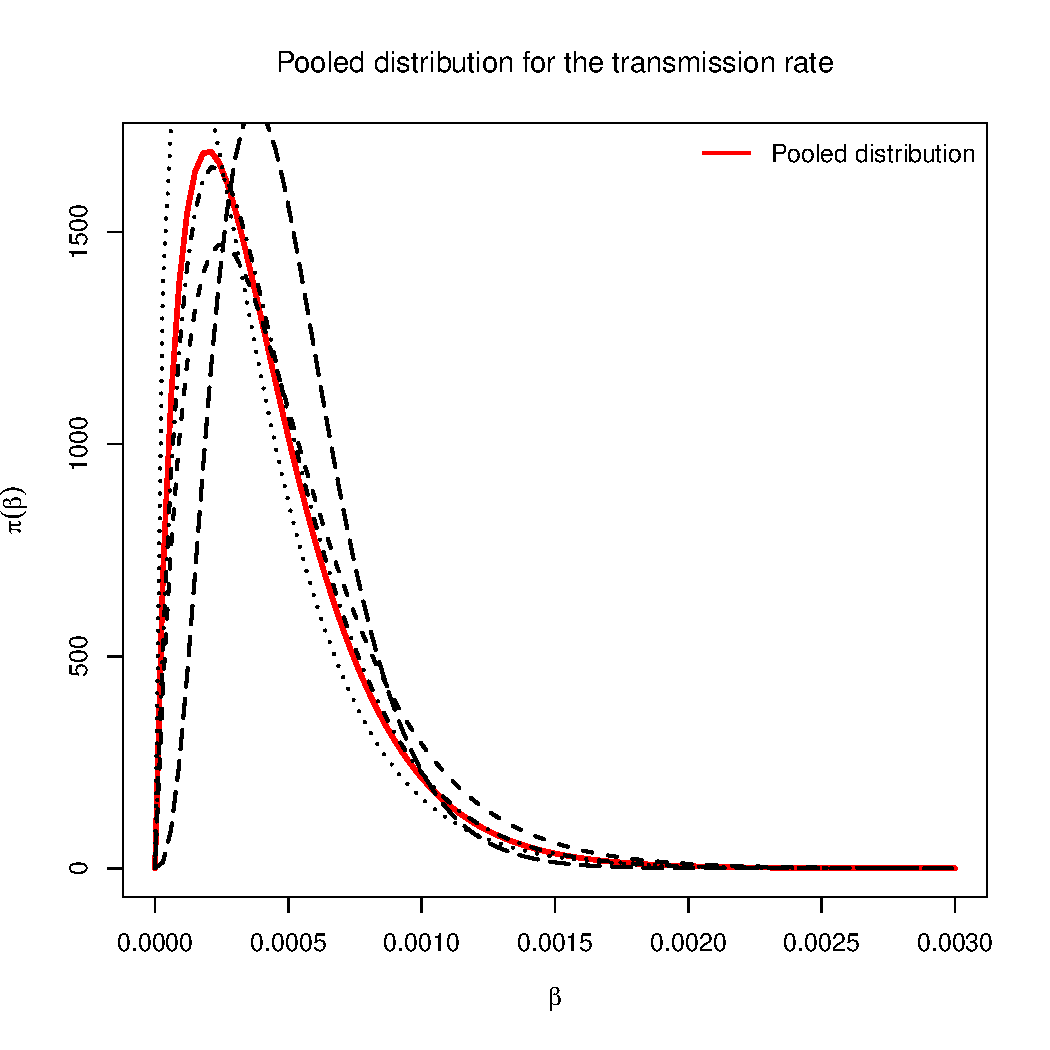
\includegraphics[scale=0.30]{figures/minKL_infection.pdf}} 
\subfigure[][]{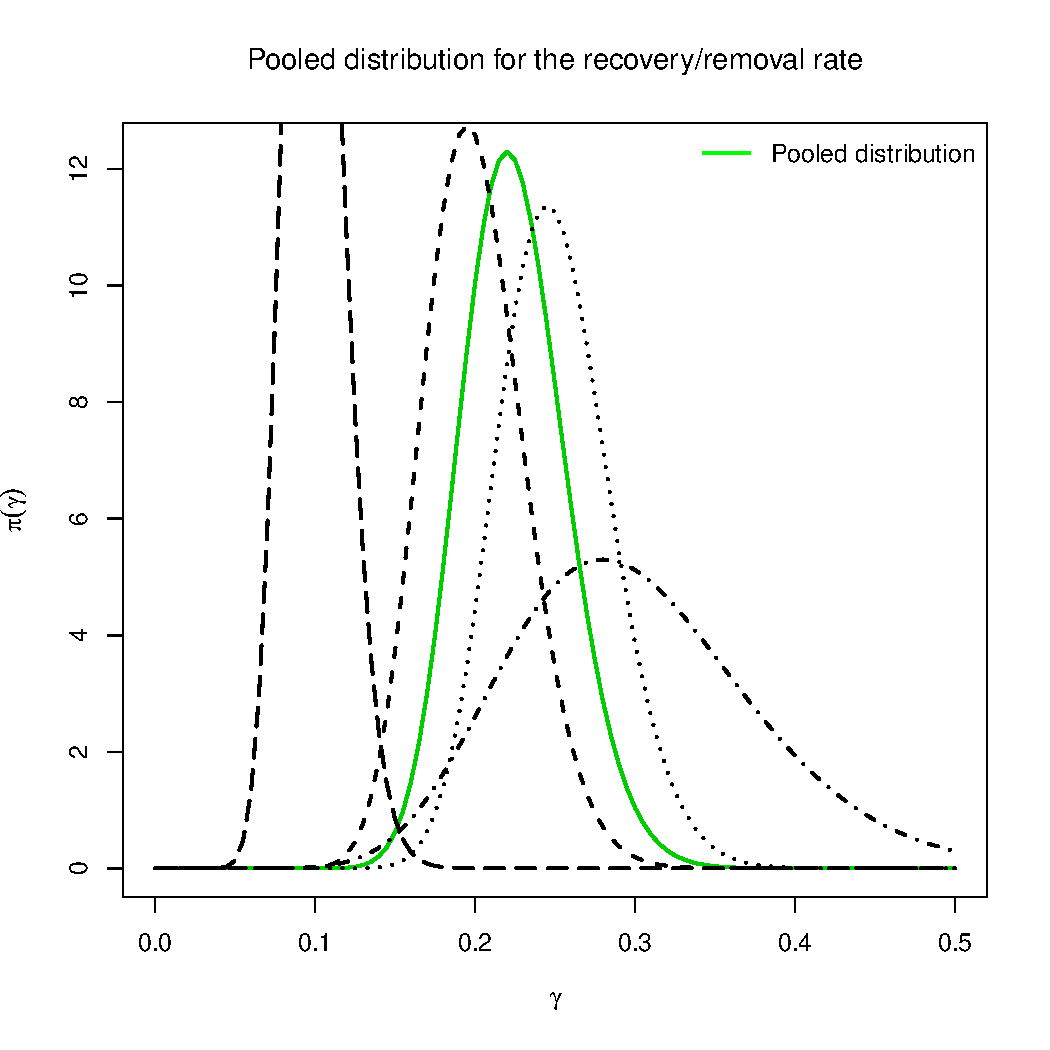
\includegraphics[scale=0.30]{figures/minKL_recovery.pdf}} 
\end{figure}
\end{frame}
%%%%%%%%%%%%%%%%%%%%%%%%%%%%%%%%%%%
%%%%%%%%%%%%%%%%%%%%%%%%%%%%%%%%%%%
\begin{frame}{Pool-then-induce}
\begin{itemize}
 \item Pool:
 \[ \pi(\beta) = Gamma(\theta_{1}^*, k_{1}^*) \]
 \[ \pi(\gamma) = Gamma(\theta_{2}^*, k_{2}^*) \]
 where $\theta^* = \sum_{i= 0}^K \alpha_i a_i$. Then
\item Induce:
\[ \pi_{1}({\cal R}_0) \propto  {{\cal R}_0}^{k_1-1} (\theta_{2}^* {\cal R}_0 + N\theta_{1}^*)^{-(k_{1}^* +  k_{2}^*)}\]
\item Nice! 
\end{itemize}
\end{frame}
%%%%%%%%%%%%%%%%%%%%%%%%%%%%%%%%%%%
%%%%%%%%%%%%%%%%%%%%%%%%%%%%%%%%%%%
\begin{frame}{Induce-then-pool}
\begin{itemize}
 \item Induce (transform) each distribution (Gamma ratio):
 \[ \pi_{i}({\cal R}_0) \propto  {{\cal R}_0}^{k_1-1} (\theta_2 {\cal R}_0 + N\theta_1)^{-(k_1 + k_2)} \]
 then
\item Pool:
\[ \pi_{2}({\cal R}_0)  \propto \prod_{i = 0}^K \pi_{i}({\cal R}_0) ^{\alpha_i}\]
\item Ugly!
\end{itemize}
\end{frame}
%%%%%%%%%%%%%%%%%%%%%%%%%%%%%%%%%%%
%%%%%%%%%%%%%%%%%%%%%%%%%%%%%%%%%%%
\begin{frame}{Dynamic model example (cont.)}
 \begin{figure}
 \begin{center}
  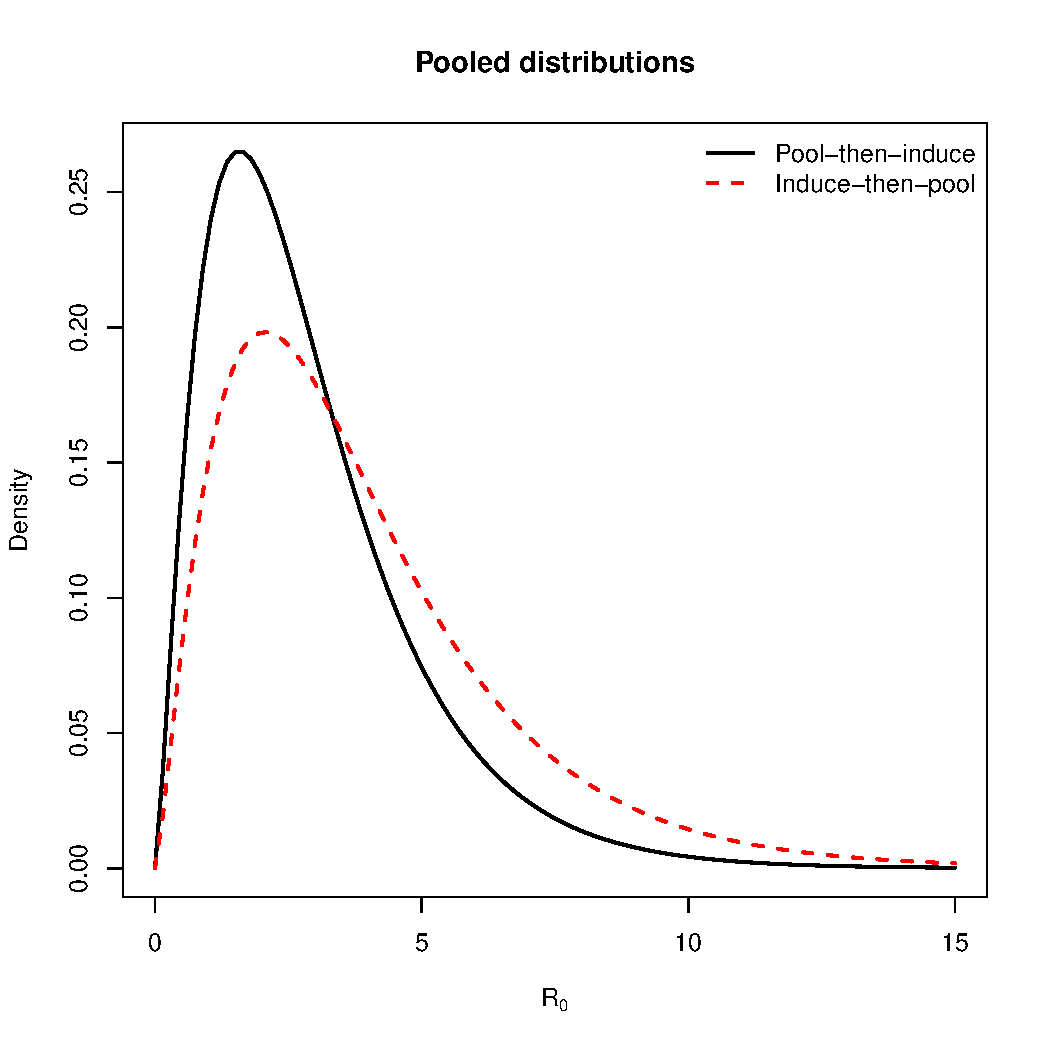
\includegraphics[scale=0.4]{figures/ItP_vs_PtI_equalWeights.pdf}
 \end{center}
  \end{figure}
\end{frame}
%%%%%%%%%%%%%%%%%%%%%%%%%%%%%%%%%%%
%%%%%%%%%%%%%%%%%%%%%%%%%%%%%%%%%%%
\begin{frame}{Thank you!}
 \begin{itemize}
  \item Thank you very much for your attention!
  \item The authors would like to thank Professor Adrian Raftery (University of Washington) for helpful suggestions.
DAMV was supported in part by Capes under Capes/Cofecub project (N. 833/15).
FCC is grateful to Funda\c{c}\~ao Getulio Vargas for funding during this project.
  \item All the necessary code and data are publicly available at~\url{https://github.com/maxbiostat/opinion_pooling}
 \end{itemize}
\end{frame}